\chapter{Modelo de minería de datos}

La necesidad de comprender los procesos biológicos que están implicados en las distintas enfermedades, a partir de la gran cantidad de datos biológicos que hay disponibles como las secuencias genómicas, los microarreglos, las interacciones proteicas, las imágenes biomédicas entre otros. Además la rápida adopción de las historias clínicas electrónicas proporciona una oportunidad de realizar investigaciones a gran escala. Por lo tanto las técnicas de minería de datos para el descubrimiento de conocimiento a partir de la obtención de información proveniente de diferentes fuentes son cada vez mas importantes en la investigación biológica y médica \cite{Wang2017}.\\

El mayor reto de la minería de datos genómicos esta en la extracción de información relevante de grandes volúmenes de datos clínicos y transformarlos en conocimiento, los mayores retos están en: a) La recolección de los datos clínicos y genómicos, b) recuperación de información relevante de datos y c) extracción de nuevos conocimientos de la información \cite{Farid2016}. \\  

Este capitulo esta organizado en análisis exploratorio de los datos que se describe en la sección 5.1, el siguiente, es el analisis textual de información clínica que es discutido en la sección 5.2 en este apartado se describe el analisis de asociación de variantes con la información clínica. Finalmente, el apartado de 5.3 se presentan las conclusiones junto con el resumen del capitulo. 

\section{Análisis exploratorio de los datos}

Se realizo el análisis exploratorio de la información contenida dentro de la base de datos.Se tomo una muestra de 250 pacientes donados por el laboratorio Genetix S.A.S de los cuales solo 228 contaban con consentimiento informado para utilizar la información con fines de investigación.\\

\begin{figure}[h!]
	\centering
	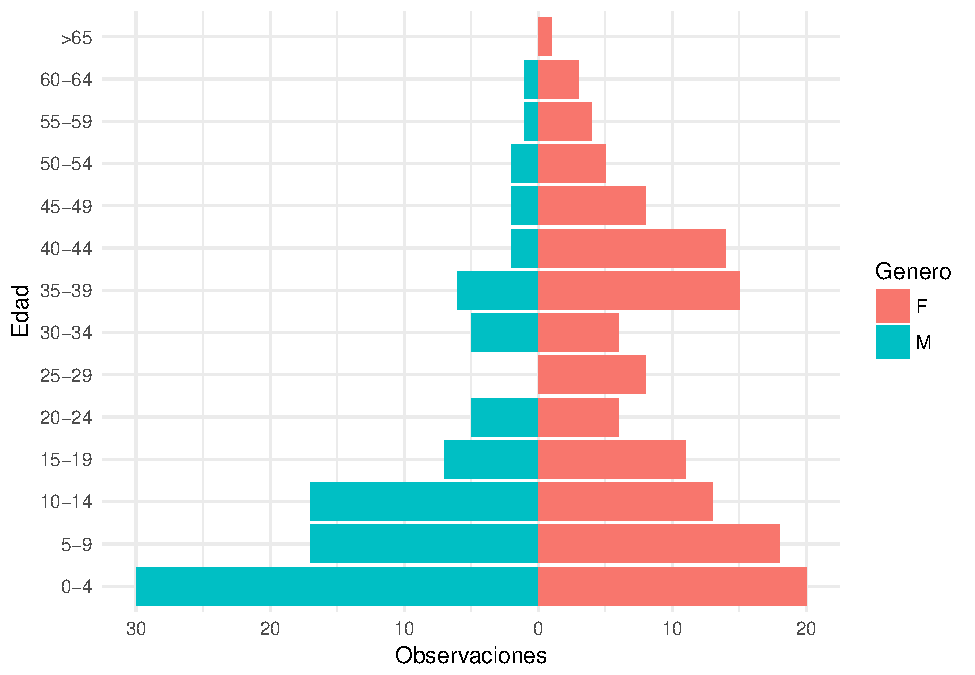
\includegraphics[width=0.5\textwidth]{Kap4/general}
	\caption{Distribución de rango de edades y géneros de los pacientes}
	\label{fig:general}
\end{figure}

\begin{figure}[H]
	\centering
	\subfigure[Distribución de variantes según su tipo.]{
		\label{f:generosgeneral}
		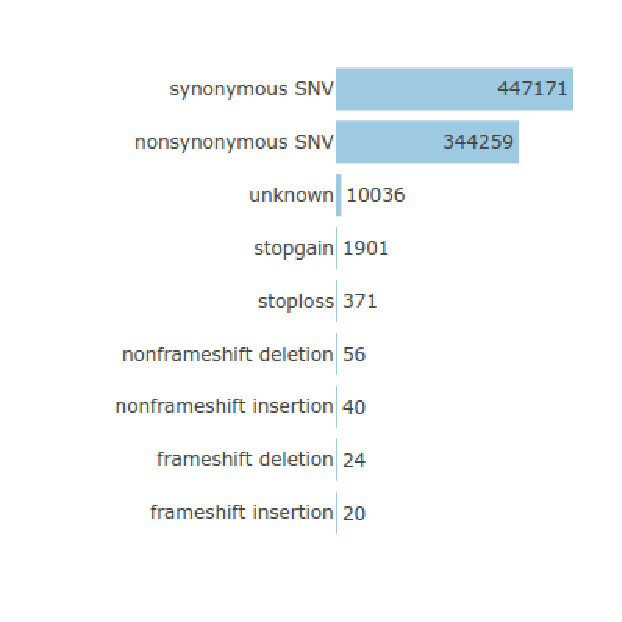
\includegraphics[width=0.35\textwidth]{Kap4/variantes.png}}
	\subfigure[Distribución de variantes por rango de edad]{
		\label{f:variantedad}
		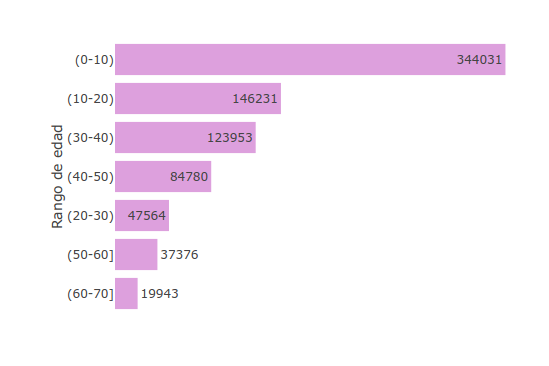
\includegraphics[width=0.55\textwidth]{Kap4/edad.png}}
	\caption{Distribución del tipo de variantes}
	\label{f:variantesgeneral}
\end{figure}

La base de datos contiene 228 pacientes de los cuales 133 son de género femenino y tienen un total de 468.485 variantes y 95 de género masculino con 345.239 de variantes obteniendo  un total de 803.878 variantes. La  figura \ref{fig:general} representa la distribución de pacientes por rango de edades y la figura \ref{f:variantesgeneral} representa la distribución de variantes según su tipo. En la figura \ref{f:generosgeneral} muestra el número de variantes que son sinónimas y no sinónimas siendo las más frecuentes en la población, a  nivel mundial se conoce que estos son lo tipos de variantes más frecuentes\cite{Fu2013}.\\

Las variantes desconocidas son el tercer tipo de variante más frecuente dado que aún existe el problema de selección del transcripto para realizar la nomenclatura adecuada de las variantes, por lo que el anotador informa que son desconocidas \cite{McCarthy2014}. La figura\ref{f:variantedad} muestra la distribución de las variantes identificadas según el rango de edad, siendo el rango con mayor número de variantes los pacientes que se encuentran entre las edades de 0 a 10 años, dado a que es la población más representada dentro de la base de datos. \\

El estado alélico de las variantes (cigocidad) que se encuentran dentro de la base de datos se dividen en heterocigotas 458639 que corresponden al 57,05\% del total de las variantes  y homocigotas 345239 que corresponden al 42,95\%. La distribución de la cigocidad de las variantes se puede explicar desde el error que se puede generar en la identificación de las variantes dado que durante el llamado  de variantes es posible que una variante homocigota se catalogue como heterocigota o si durante el proceso de secuenciación se identifican erróneamente los nucleótidos \cite{Babraham2016}\cite{Pirooznia2014}. 


\section{Análisis textual de información clínica.}

 
\subsection{Preprocesamiento.}

El proceso de limpieza y nacionalización de texto se realizo de la siguiente manera:

 \begin{enumerate}
 	\item Remoción de stop words en español, tildes y caracteres especiales como  la letra ñ y todos los documentos se unificaron en letras minúsculas.
 	\item Teniendo en cuenta la información clínica se creo un diccionario de sinónimos, donde se reemplazaron palabras que hacen referencia a una misma característica.
 	\item Calculo de la frecuencias de palabras dentro de los documentos. 
 	\item Se removieron las palabras pam,pacientes, secuenciación y gen dado que no son un factor diferenciador de los documentos.  	  
 \end{enumerate}

\subsection*{Resultados}

Los resultados que se obtuvieron para la frecuencia de palabras fueron seno, cáncer, síndrome, sospecha y años. La figura \ref{fig:sin} muestra las primeras 30 palabras más frecuentes y la nube de palabras de todos los documentos.\\

\begin{figure}[]
	\centering
	\subfigure[Nube de palabras]{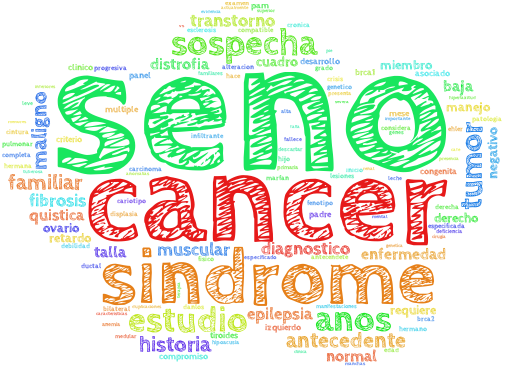
\includegraphics[width=60mm]{Kap4/sin_stop}}
	\subfigure[Frecuencia de términos]{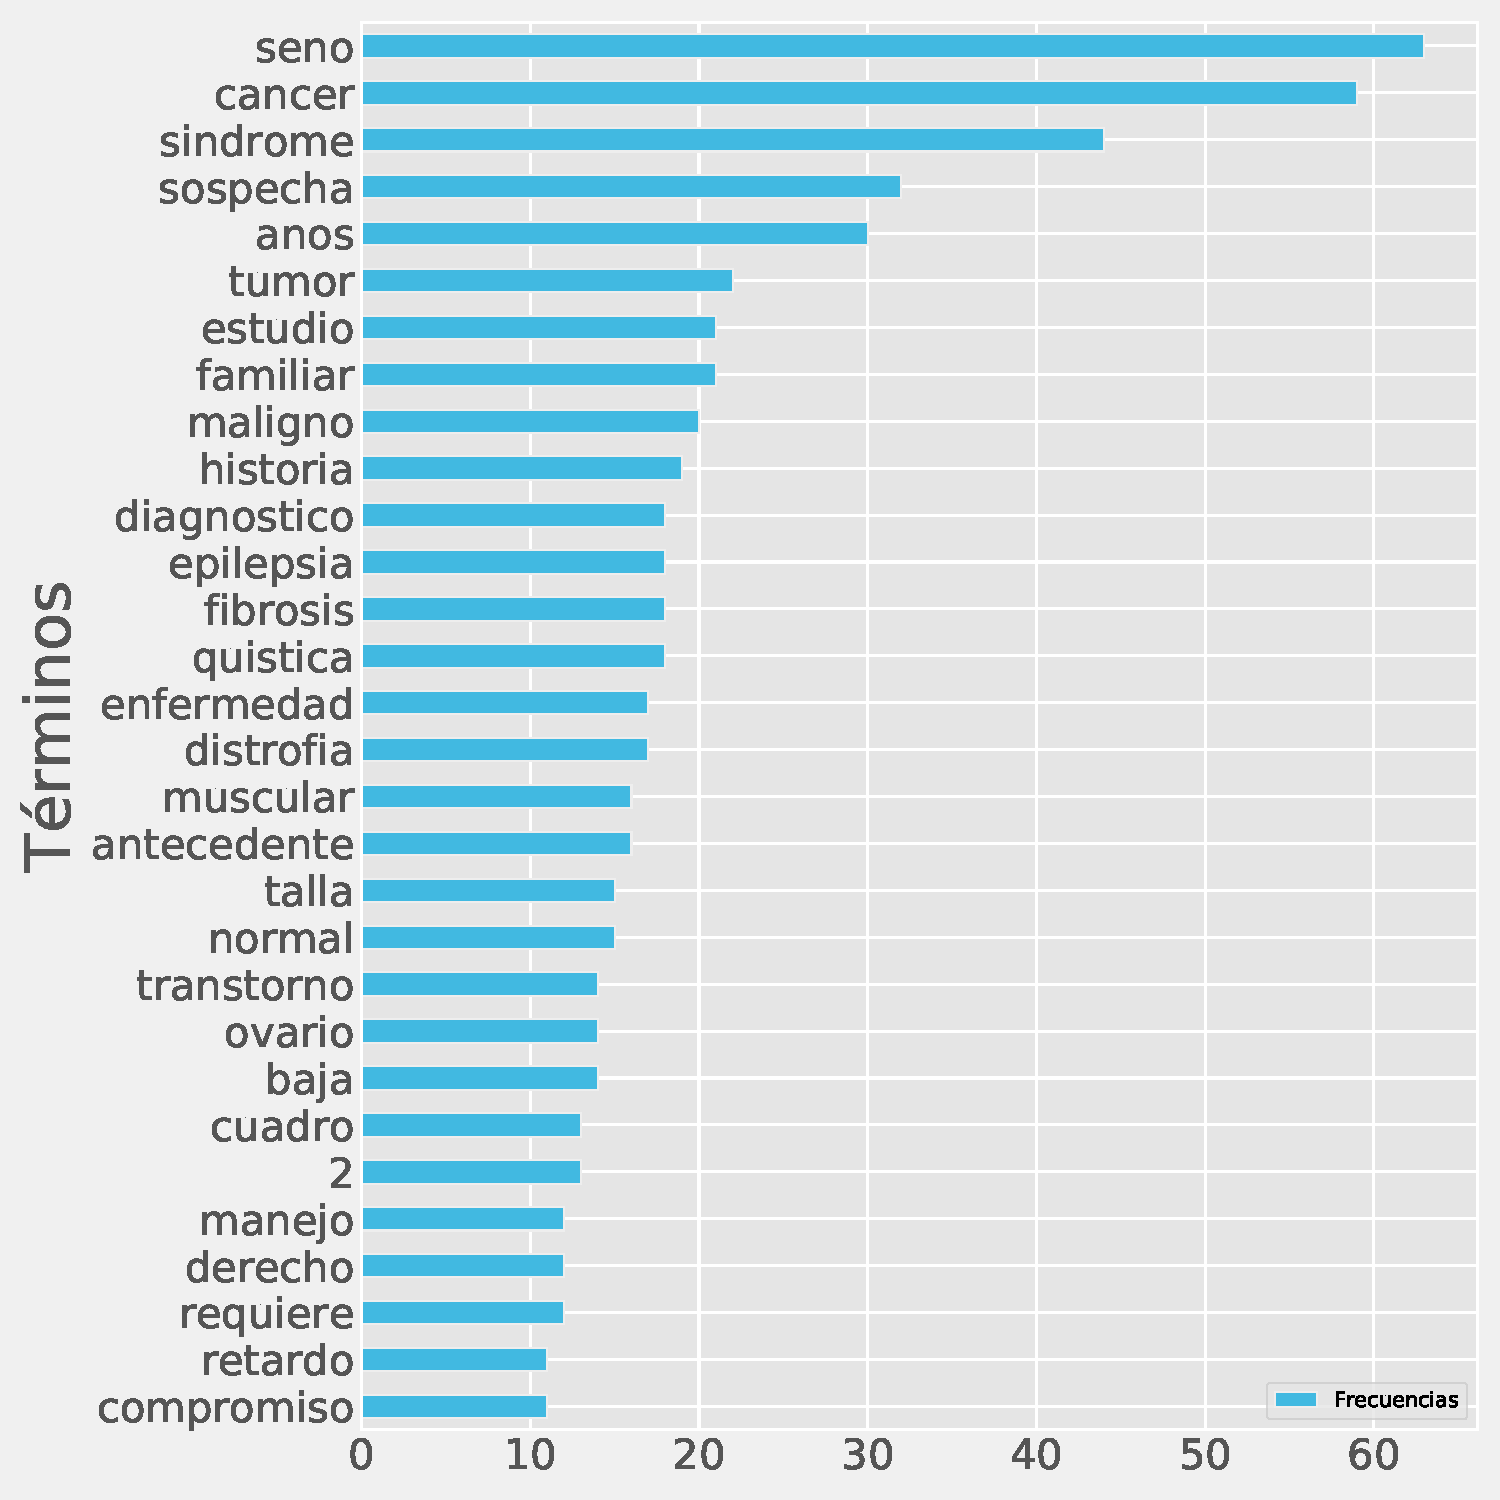
\includegraphics[width=60mm]{Kap4/frecuecias.pdf}}
	\caption{Frecuencias sin stop words y palabras sinónimas} \label{fig:sin}
\end{figure} 

Las frecuencia de palabras nos muestra las principales características de la información clínica siendo las palabras cáncer y seno los principales fenotipos, también se encuentra la palabra síndrome que puede asociarse a diferentes  enfermedades y la palabra sospecha hace referencia a diagnósticos ambiguos que pueden tener los pacientes, una de las contribuciones de la secuenciación es que basado en el fenotipo puede ayudar a un diagnóstico,entre diferentes síntomas y síndromes que pueden ser aplicados a enfermedades raras y complejas\cite{Tetreault2015a}.

\subsection{Grupos de características clínicas.}

En los procesos médicos, la relación entre los factores que pueden afectar la salud juega un papel importante. Una de las relaciones más comunes es la relación entre los genes y las enfermedades donde la secuenciación de exones tiene una alta aplicabilidad. Pero la identificación manual de este tipo de relaciones es compleja dada la cantidad de características que se pueden presentar como el diagnóstico propio de la enfermedad y/o la respuesta a los tratamientos \cite{Kawashima2017}.

La minería texto y puede ser aplicado al análisis en la medicina, donde el clustering (agrupamiento) puede ser considerado el método más importante que se utiliza en aprendizaje de maquina no supervisado que ha sido aplicado a diferentes problemas\cite{Kawashima2017}, teniendo en cuenta que no de los objetivos del agrupamiento de datos, es la  identificación de grupos naturales en datos sin etiquetas\cite{Jain2010}.

Partiendo de lo anterior el presente trabajo se implemento un modelo de agrupamiento para identificar grupos de características clínicas con la siguiente metodología:

\begin{enumerate}
	\item Cálculo de la matriz tf-idf y se normalizo. 
	\item Estimación de el número de k optimo.
	\item Implementación del algoritmo k-means.
	\item Validación de los clusters.
	\item Análisis de resultados. 	  
\end{enumerate}

\subsection{Resultados}

El cálculo de la matriz tf-idf, se realiza a partir de frecuencia invertida con la ecuación ${idf}_i = \log_2 \frac{|D|}{|\{d \mid t_i \in d\}|}$ siendo $|D|$ lo que denota el número total de documentos y donde $|\{d\mid t_i \in d\}|$ en  que $t_1$ aparece, la matriz de tf-idf es calculada a partir de la multiplicación de la frecuencia de términos y la frecuencia invertida $\mathit{tf}_{i,j} \cdot \mathit{idf}_i$ \cite{Buckley1988}. 
La figura \ref{fig:IDFTF} representa la matriz IDF-TF de las palabras que se encuentran dentro de la base de datos.  

\begin{figure}[H] 
	\centering
	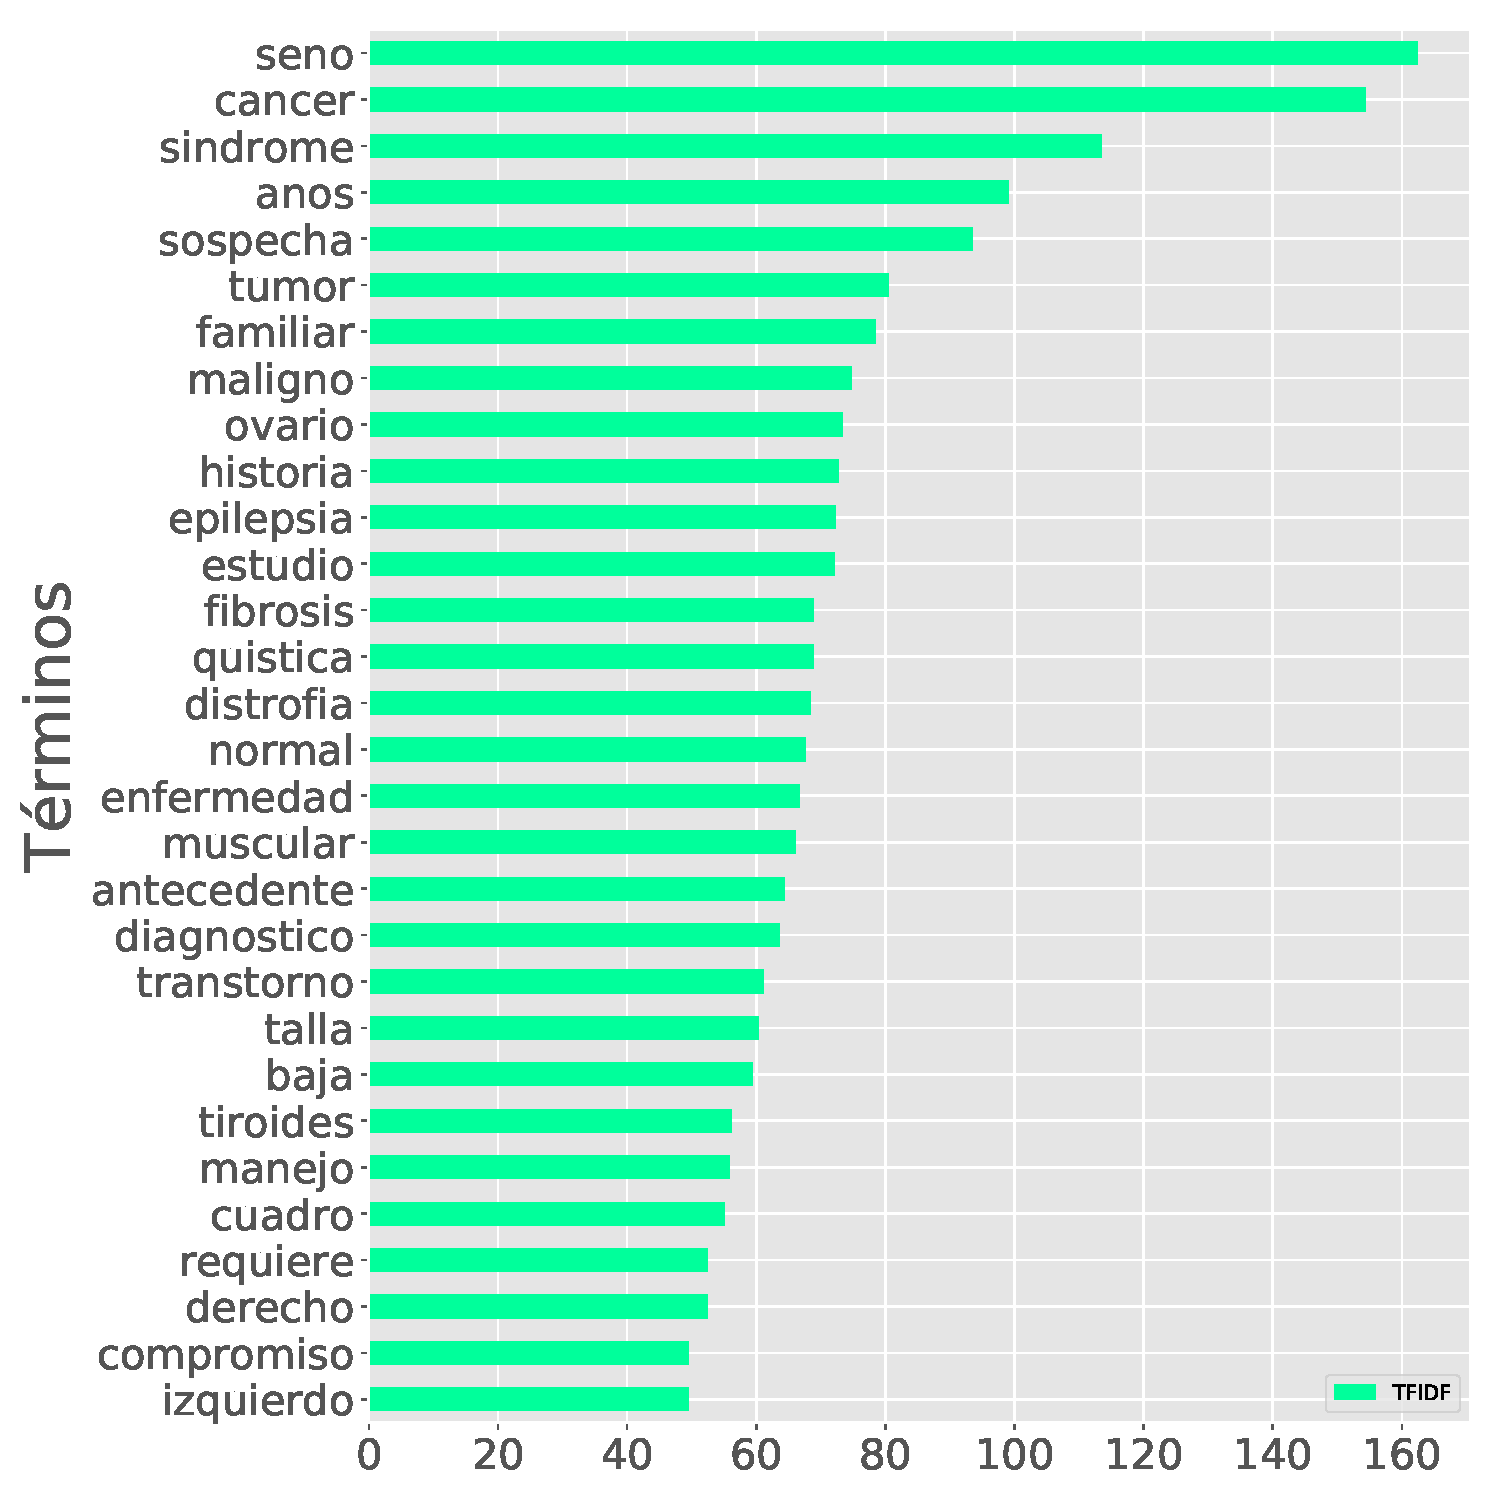
\includegraphics[width=0.5\textwidth]{Kap4/tfidf.pdf}
	\caption{TFIDF} 
	\label{fig:IDFTF}
\end{figure}

Selección de el número optimo de K se ejecuto el algoritmo k-means obteniendo cinco clusters:

\begin{figure}[H] 
	\centering
	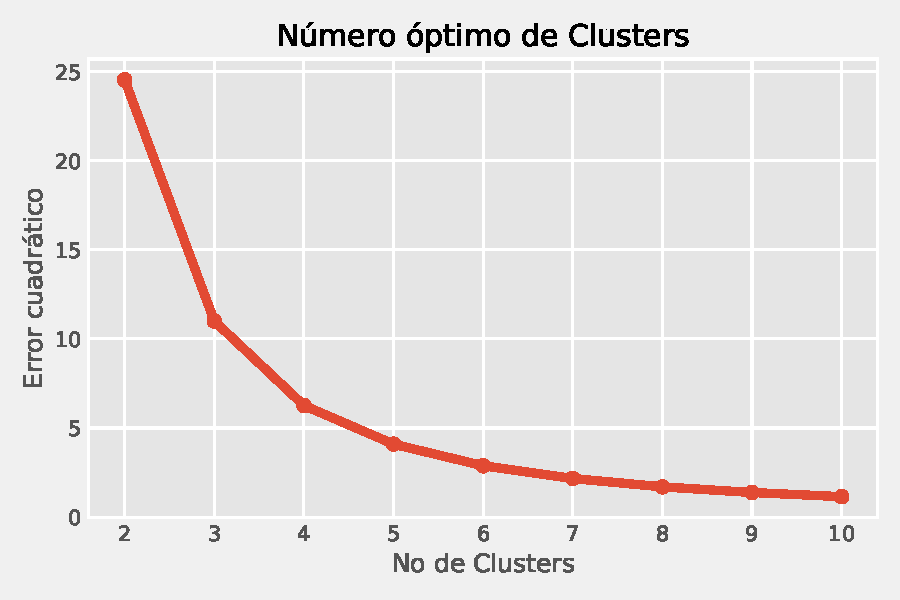
\includegraphics[width=0.5\textwidth]{Kap4/Clusters.pdf}
	\caption{Número optimo de clusters} 
	\label{fig:Clusters}
\end{figure}

\begin{figure}[H] 
	\centering
	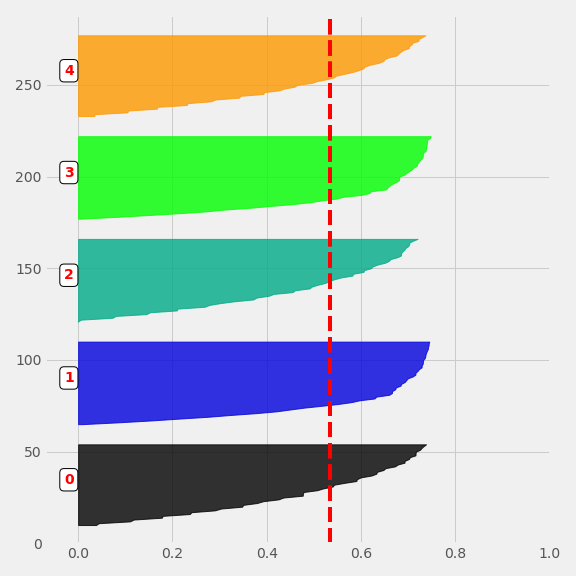
\includegraphics[width=0.8\textwidth]{Kap4/S}
	\caption{Valor Silueta de cada cluster} 
	\label{fig:S}
\end{figure}

\begin{figure}[H]
	\centering
	\subfigure[Nube de palabras]{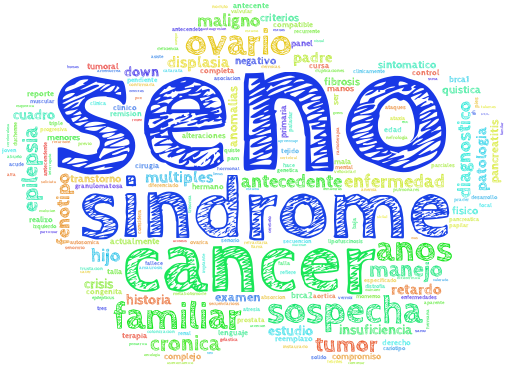
\includegraphics[width=80mm]{Kap4/cluster1}}
	\subfigure[Rango de edad en decadas]{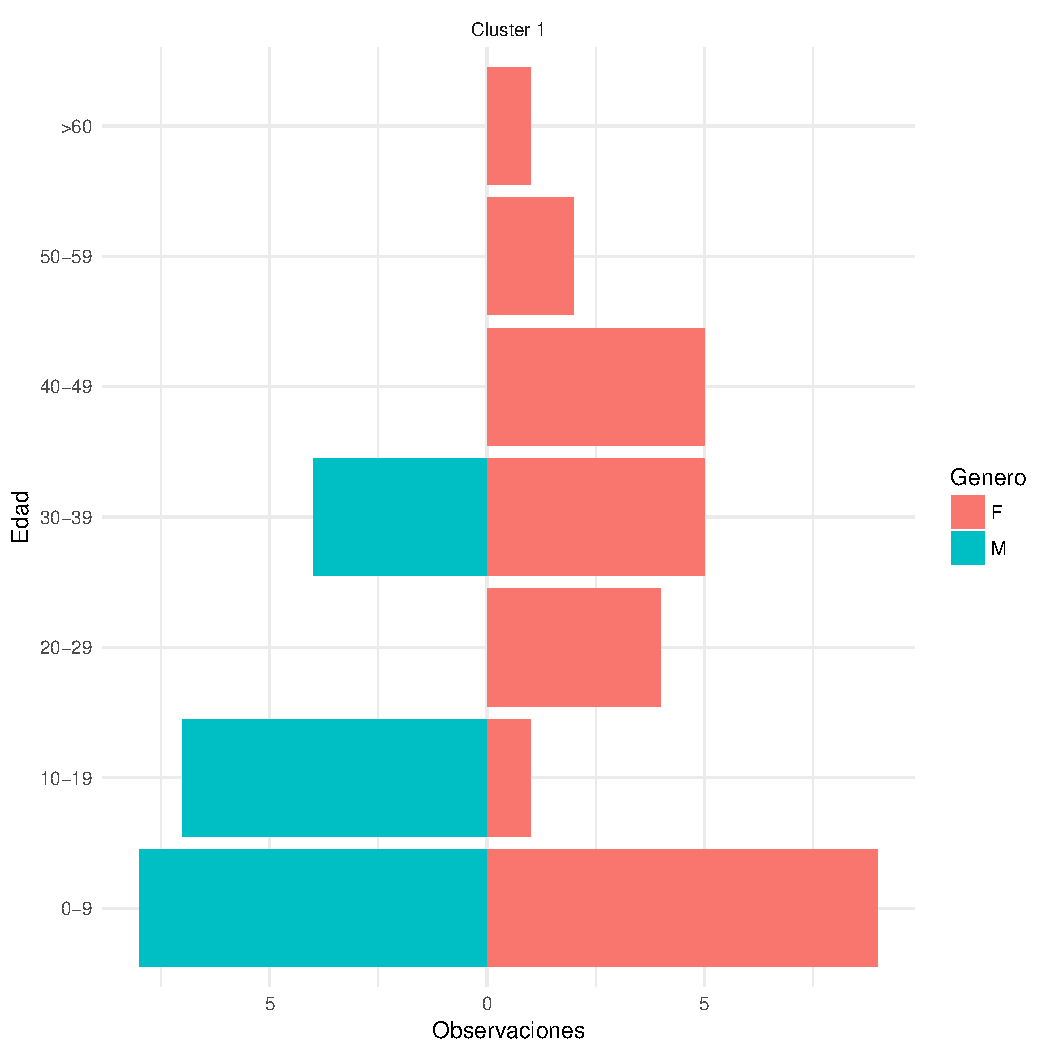
\includegraphics[width=70mm]{Kap4/edadsexocluster1}}
	\caption{Cluster 1} \label{fig:c1}
\end{figure}

La figura \ref{fig:c1} representa el clúster 1 con la información clínica que presenta en (a) tenemos la frecuencia de palabras, siendo seno,síndrome y cáncer son las palabras más frecuentes, junto con ovario y familiar.

\begin{figure}[H]
	\centering
	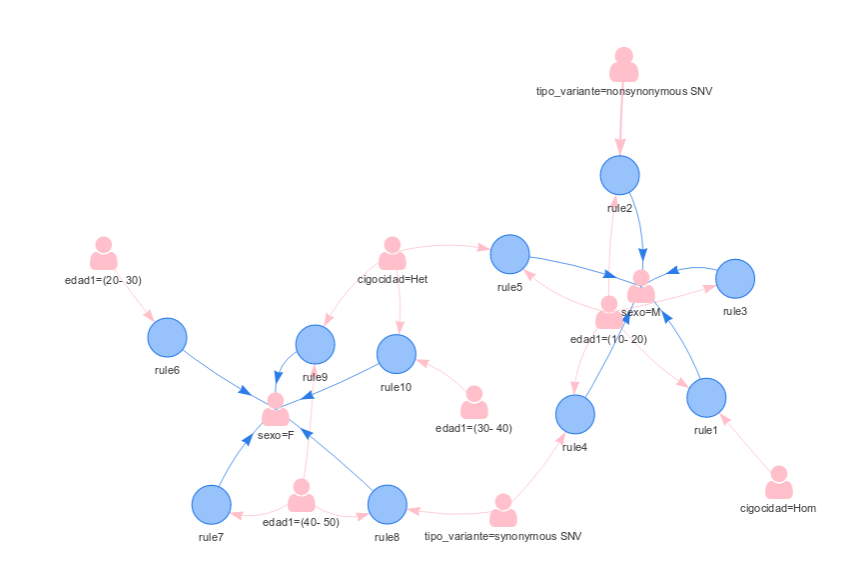
\includegraphics[width=0.9\textwidth]{Kap4/reglasc1}
	\caption{Reglas de asociación del cluster 1} \label{fig:reglas}
\end{figure}

Las primeras 10 reglas obtenidas se representan mediante la figura \ref{fig:reglas} que muestra la asociación de dos tipos de variantes dentro del clúster 1 con el genero masculino donde se tiene que el tipo de variante es no sinónima, son pacientes de edad entre 10 y 20 años, el estado alélico de las variantes es homocigoto, para este grupo se observa una alta diferencia en las reglas ambos géneros, 


\begin{figure}[H]
	\centering
	\subfigure[Nube de palabras]{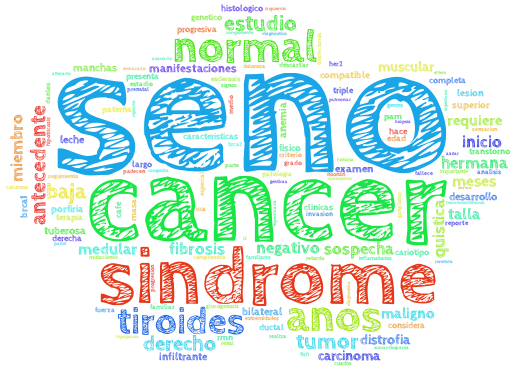
\includegraphics[width=60mm]{Kap4/cluster2}}
	\subfigure[Rango de edad en decadas]{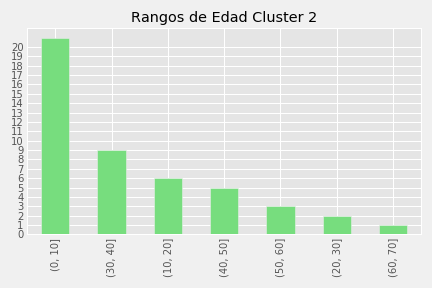
\includegraphics[width=60mm]{Kap4/edadcluster2}}
	\subfigure[Género]{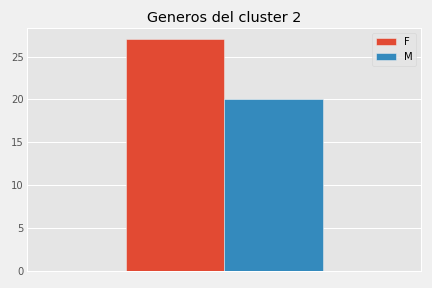
\includegraphics[width=60mm]{Kap4/Cluster2G}}
	\caption{Cluster 2} \label{fig:c2}
\end{figure}

% Please add the following required packages to your document preamble:
% \usepackage{booktabs}
% Please add the following required packages to your document preamble:
% \usepackage{booktabs}
\begin{table}[]
	\centering
	\caption{My caption}
	\label{my-label}
	\begin{tabular}{@{}|c|c|@{}}
		Rango de Edad & No. de pacientes . \\ 
		0-10          & 15                 \\
		10-20         & 9                  \\
		20-30         & 3                  \\
		30-40         & 7                  \\
		40-50         & 7                  \\
		50-60         & 2                  \\ 
		60-70         & 2                  \\
		Total         & 45                 \\
	\end{tabular}
\end{table}

donde...

\begin{figure}[H]
	\centering
	\subfigure[Nube de palabras]{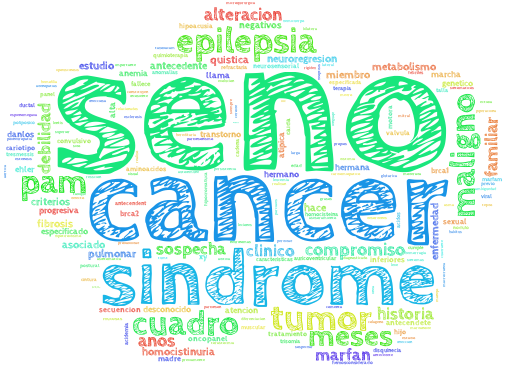
\includegraphics[width=60mm]{Kap4/cluster3}}
	\subfigure[Rango de edad en decadas]{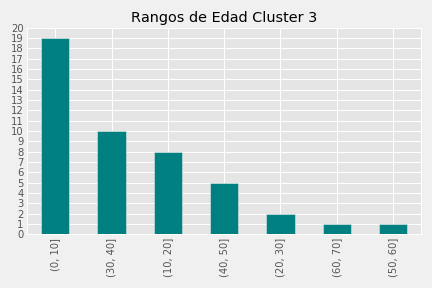
\includegraphics[width=60mm]{Kap4/edadcluster3}}
	\subfigure[Género]{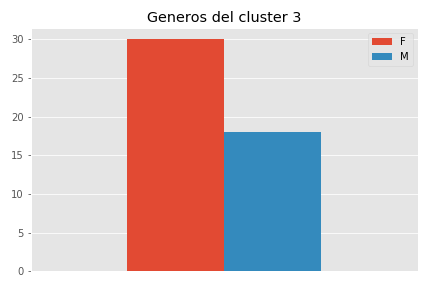
\includegraphics[width=60mm]{Kap4/Cluster3G}}
	\caption{Cluster 3} \label{fig:c3}
\end{figure}

Donde ...

\begin{figure}[H]
	\centering
	\subfigure[Nube de palabras]{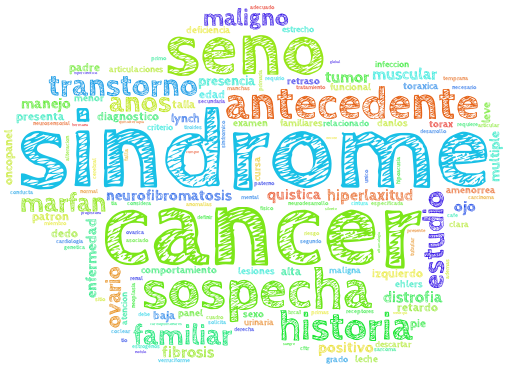
\includegraphics[width=60mm]{Kap4/cluster4}}
	\subfigure[Rango de edad en decadas]{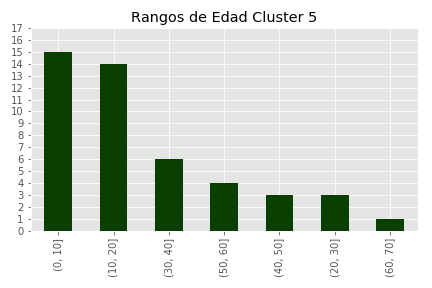
\includegraphics[width=60mm]{Kap4/edadcluster4}}
	\subfigure[Género]{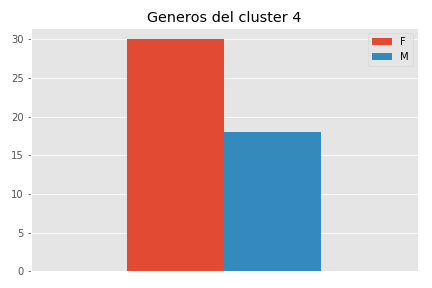
\includegraphics[width=60mm]{Kap4/Cluster4G}}
	\caption{Cluster 4} \label{fig:c4}
\end{figure}

Donde 

\begin{figure}[H]
	\centering
	\subfigure[Nube de palabras]{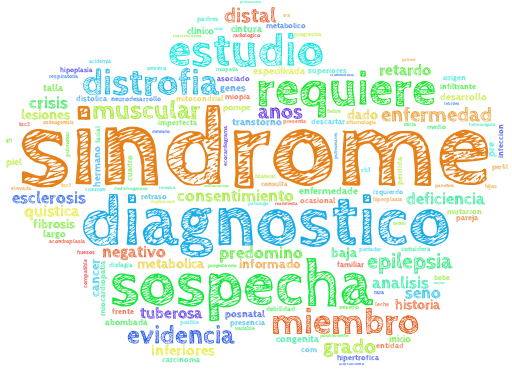
\includegraphics[width=60mm]{Kap4/cluster5}}
	\subfigure[Rango de edad en decadas]{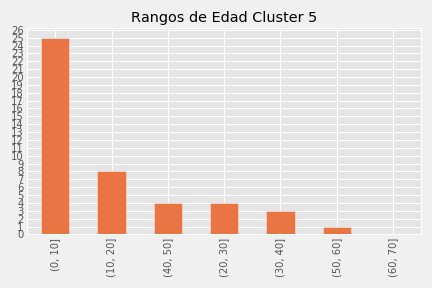
\includegraphics[width=60mm]{Kap4/edadcluster5}}
	\subfigure[Género]{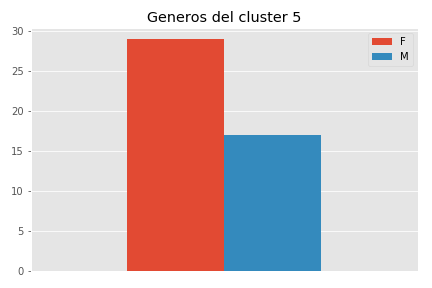
\includegraphics[width=60mm]{Kap4/Cluster5G}}
	\caption{Cluster 5} \label{fig:c5}
\end{figure}
